\documentclass{article}

\usepackage{graphicx}

\title{AI Homework 4}
\author{Connor Taffe}

\begin{document}
  \maketitle

  The best $k$ value was $k=7$, with an accuracy probability of $0.73743$.

  {\centering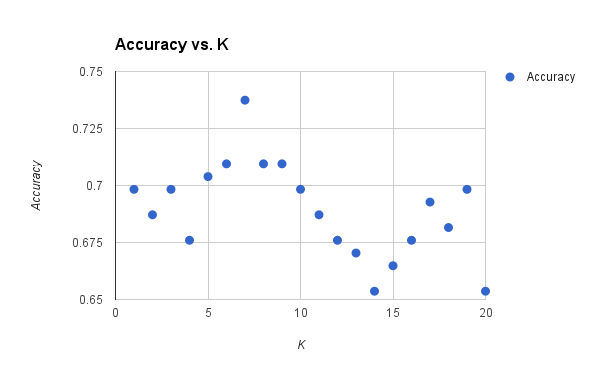
\includegraphics[width=\textwidth]{image}}

  \section{Compiling and Executing}

  I suppose open {\tt main.cc} in Visual Studio. Click the run button.

  \section{Description}

  The tradeoffs between the value of $k$ and the accuracy has to do with the number of samples and the size of the dataset. Since I calculated the distance between every node and the testing node before taking the first $k$ nodes and averaging means that because of my hugely inefficient approach, there is no further penalty in performance of averaging more $k$ (there is, but it is an add-loop, which is extremely minimal). What one wants to do is take the maximum $k$ nodes in a locality, which depends highly upon the size of the dataset, and would benefit from wieghting the data. One could hypothesize that a $k$ equal to the size of the dataset and weighted properly would produce the best results, but since the weighting would make some nodes (far away) have a very small effect, the best approach would be to have a variable $k$ which lops off such insignificant weighted nodes.

  The static $k$ really only works well with a very dense homogenized dataset. Sets with different sparsenesses would work poorly.


\end{document}
